\begin{abstract}
Recognizing a cricket shot from one frame can be difficult when the bat is blurred or the stroke has not yet developed. We study a small, CPU-only system for classifying trimmed videos into eight shot categories. Our proposed representation combines ordered averages of early, middle and late frame embeddings with their temporal difference and spread. It uses a frozen ImageNet MobileNetV2 encoder and a class-balanced linear classifier. The contribution is a compact, inspectable design and a controlled evaluation of its components, rather than a new backbone or a claim of state-of-the-art performance. We evaluate 562 real clips with source groups kept disjoint across training, validation and test sets. The proposed model obtains 30.2\% accuracy and 21.3\% macro F1 on 116 held-out clips, compared with 19.8\% and 18.6\% for a middle-frame baseline. The proposed representation exceeds the middle-frame macro F1 by 2.7 percentage points. The local demo shows the sampled sequence, all class scores and a validation-chosen review decision. Results and limitations are supported by saved predictions and reproducible code.
\end{abstract}

\section{Introduction}
A cricket highlight is useful to a viewer, but it does not automatically provide a searchable record of the strokes played. Recognizing shots could help organize a video collection or retrieve examples for a discussion of technique. Here, the input is one short video containing a batting shot. The output is one of the dataset's eight labels and an indication of whether the prediction needs review. We do not estimate runs, judge execution quality, locate shots in a full match or provide coaching advice.

The difficult cases are often visually similar. An on drive and an off drive can share a stance and follow-through, while the important bat-ball interaction may occupy only a few frames. Broadcast graphics, clothing and camera position may also provide shortcuts unrelated to the stroke. A model can therefore look convincing on a random clip split and still fail on a different source video.

Our working hypothesis is that a cheap temporal summary can preserve useful stroke progression without training a recurrent network on a small dataset. We divide nine sampled embeddings into three ordered bins, retain their means, and add a late-minus-early difference and temporal standard deviation. This descriptor is deliberately simple enough to explain and ablate.

The course contribution has two parts. First, we implement and test this particular phase/difference/spread representation with a fixed broadcast crop against a single frame and unordered pooling under the same protocol. Second, we connect the classifier to an offline interface that exposes uncertainty and real failure cases. Temporal segmentation, transfer learning and confidence rejection already exist. We do not claim to have invented them, and this study does not establish that our combination is new to the research literature.

\section{Related work}
\textbf{Cricket recognition.} Hoque et al.'s KUCricShot provides a four-shot dataset, as documented by the authors' repository~\cite{kucricshot}. Kang's cricket baseline study compares spatial and temporal models, including recurrent and attention-based approaches~\cite{kang}. These works establish that cricket recognition and temporal modeling are existing research topics. Their data and evaluation differ from ours, so their published percentages are not entries in our comparison table. We did not run or reuse their implementations.

\textbf{Efficient visual and temporal representations.} MobileNetV2 uses inverted residuals and linear bottlenecks to support efficient vision models~\cite{sandler}. We use the public ONNX Model Zoo weights~\cite{onnxmodel} as a fixed image encoder. Temporal Segment Networks combine sparse temporal sampling with video-level supervision~\cite{wang}. Our use of temporal bins follows this broad motivation, but uses fixed pooled embeddings and a linear head. It is not a reproduction of TSN and contains no optical flow or learned attention.

\textbf{Confidence and review.} Guo et al. study calibration and scalar temperature scaling~\cite{guo}. We use a validation-fitted temperature. Selective classification studies the trade-off between coverage and prediction error~\cite{geifman}. Our review rule is a finite validation heuristic, not their guaranteed-risk procedure. It also cannot certify that an uploaded clip is cricket or belongs to a known class.

\section{Dataset and evaluation protocol}
\subsection{Data provenance and label scope}
We downloaded version 1 of \emph{CRICKET\_SHOTS} from Kaggle user \texttt{amittalmale}~\cite{dataset}. The archive SHA-256 and public metadata are preserved with the project. It contains 562 AVI files in eight label folders. The uploader supplies no detailed annotation or cropping protocol. We retain the upstream labels and do not claim that the group collected or independently relabeled these videos. Kaggle declares CC0, but we have not verified rights in the underlying broadcasts. All displayed cricket frames come from these clips.

Table~\ref{tab:data} gives the actual split. The largest class has 159 examples and the smallest has 21. The \emph{unorthodox} label is broad and does not correspond to one precise batting motion. These properties make macro F1 and per-class recall important companions to overall accuracy.

\begin{table}[t]
\centering\small
\begin{tabular}{lrrrr}
\toprule
Label & Train & Val. & Test & All \\
\midrule
Cut & 23 & 10 & 8 & 41 \\
Defence & 16 & 6 & 3 & 25 \\
Glance & 22 & 11 & 8 & 41 \\
Off drive & 76 & 32 & 29 & 137 \\
On drive & 95 & 29 & 35 & 159 \\
Pull & 44 & 29 & 23 & 96 \\
Sweep & 25 & 11 & 6 & 42 \\
Unorthodox & 16 & 1 & 4 & 21 \\
Total & 317 & 129 & 116 & 562 \\
\bottomrule
\end{tabular}
\caption{Clip counts from the prepared manifest. All eight labels occur in each set, but validation has only one unorthodox clip.}
\label{tab:data}
\end{table}


\subsection{Source grouping and audit}
Filenames identify a highlight source and a pair of frame indices. We remove the indices, normalize punctuation and title words, and standardize team pair names. In particular, two Ireland/Oman titles merge into one conservative source group. This produces 25 normalized title groups from 26 original titles. Clips sharing a file checksum stay together. We also compare first, middle and last sampled frames across sources with 64-bit perceptual hashes. Pairs with mean Hamming distance at most four and maximum distance at most six join the same split group.

The audit found 0 exact duplicate files, 0 qualifying cross-source perceptual pairs, and 0 decoding failures. There are 25 final split groups. This is a practical leakage check, not proof that every near duplicate has been detected. Source titles do not identify individual players or all camera cuts. The split therefore supports a claim about held-out source groups in this archive, not unseen players, all future matches or independent broadcasters.

We use five stratified group folds with shuffle seed 17. Fold 0 is test, fold 1 is validation and the other three are training. The resulting sets contain 317, 129 and 116 clips from 14, 6 and 5 groups. Source names, union groups and exact file hashes do not overlap across sets. We report one fixed holdout, not a five-fold cross-validation average.

\section{Proposed method}
\begin{figure*}[t]
\centering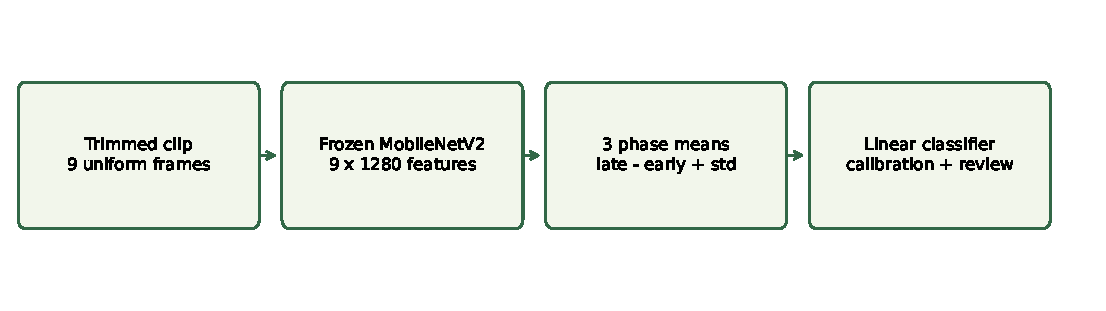
\includegraphics[width=.98\textwidth]{method_overview.pdf}
\caption{The implemented pipeline. Only the linear classifier learns from the cricket training split. Temperature and the review threshold use validation clips. The three bins are positions in the sampled sequence, not detected preparation, impact or follow-through events.}
\label{fig:method}
\end{figure*}

\subsection{Frames and frozen visual features}
We decode each clip sequentially and sample nine frame indices uniformly, including both endpoints. Frames are bounded to a 640 by 480 preview box. A fixed region $x\in[0.30W,0.70W]$, $y\in[0.02H,0.65H]$ emphasizes the usual upper-center batter position and removes much of the scoreboard and bowler. We resize and center-crop this region to 224 by 224 without stretching the aspect ratio. RGB values use ImageNet mean $(0.485,0.456,0.406)$ and standard deviation $(0.229,0.224,0.225)$. This is a camera-layout assumption, not a person detector. It can remove the batter in a different view. The same function runs during training and demo inference.

The pretrained MobileNetV2 global average pooling layer produces $f_t\in\mathbb{R}^{1280}$. We remove the ImageNet classification head and normalize each embedding, $u_t=f_t/\max(\|f_t\|_2,10^{-12})$. The encoder is frozen. This avoids claiming that an ImageNet classifier already recognizes cricket shots.

\subsection{Ordered phase, difference and spread descriptor}
For $k=1,2,3$, the phase mean is
\begin{equation}
\mu_k=\frac{1}{3}\sum_{t=3k-2}^{3k}u_t.
\end{equation}
Let $\sigma$ be the elementwise population standard deviation of the nine normalized embeddings. The proposed descriptor is
\begin{equation}
z=\operatorname{L2Norm}([\mu_1;\mu_2;\mu_3;\mu_3-\mu_1;\sigma]).
\end{equation}
It has 6,400 dimensions. Ordered means retain coarse progression. The difference encodes the direction of change, while spread summarizes how much the representation varies. The difference is algebraically redundant with the phase means, so it adds no new information to an unrestricted linear model. Its effect here is to change the feature weighting and effective regularization. The standard deviation can add information beyond the phase averages. We evaluate their joint addition and do not isolate either effect.

The classifier is an L2-regularized multinomial logistic regression with balanced class weights. Its eight outputs contain 51,208 trainable coefficients and intercepts. There is no recurrent network, pose detector, ball tracker, attention module or bat localization stage.

\subsection{Calibration and review decision}
For logits $a_c$, the calibrated probability is
\begin{equation}
p(c\mid z)=\frac{\exp(a_c/T)}{\sum_j\exp(a_j/T)}.
\end{equation}
We choose $T\in[0.1,10]$ by minimizing validation negative log likelihood. A positive scalar temperature changes confidence but preserves the top class. The review rule accepts only if $\max_c p(c\mid z)\geq\tau$. Candidate thresholds range from 0.30 to 0.95 in steps of 0.05. We take the lowest threshold reaching 90\% validation accuracy with at least 20\% coverage and ten accepted clips. If none qualifies, the explicit fallback is 0.80. No test label participates in either choice. Reusing one validation split for regularization, calibration and threshold selection may overfit it, especially for rare classes.

\section{Experiments and results}
\subsection{Implementation and controls}
Each descriptor uses exactly the same frozen embeddings and source split. We compare: a training-majority predictor, a 96-bin hue/saturation histogram, the middle sampled frame (1,280 dimensions), a mean across all frames (1,280), three ordered phase means (3,840), and the proposed descriptor (6,400). All learned heads use balanced logistic regression with the same $C\in\{0.1,1,10,100\}$ grid. Validation macro F1 selects $C$, with smaller values winning ties. There is no cricket-specific pretraining, fine-tuning, synthetic data or training augmentation.

The full-frame pilot specification preceded test scoring. That pilot achieved 18.1\% test accuracy and 17.7\% macro F1 for the proposed descriptor. After inspecting its aggregate scores and sample footage, we added the fixed crop to address the small batter scale. The crop bounds were then fixed before ROI scoring. We retained the source split, so the final comparison is exploratory on a reused holdout, not an untouched confirmatory test. Original pilot predictions remain available. The proposed descriptor stays deployed even if an ablation performs better. Training uses scikit-learn and inference uses ONNX Runtime on CPU with two intra-operation threads. Numeric NPZ/JSON classifier export avoids loading Python pickles. The measured environment and dependency versions are saved with the results.

\subsection{Recognition and ablations}
\begin{table}[t]
\centering\small
\begin{tabular}{lrrr}
\toprule
Representation & $C$ & Acc. (\%) & F1 (\%) \\
\midrule
Training majority & -- & 30.2 & 5.8 \\
Color histogram & 0.1 & 9.5 & 7.9 \\
Middle frame & 10 & 19.8 & 18.6 \\
Temporal mean & 10 & 18.1 & 17.9 \\
Ordered phases & 10 & 18.1 & 16.8 \\
Phase + diff./std. & 100 & 30.2 & 21.3 \\
\bottomrule
\end{tabular}
\caption{All learned heads select regularization by validation macro F1. Final visual models use the same fixed ROI and split. Color uses the full frame. F1 is macro-averaged.}
\label{tab:results}
\end{table}

Table~\ref{tab:results} shows that the proposed representation has 30.2\% accuracy and 21.3\% macro F1. The proposed representation exceeds the middle-frame macro F1 by 2.7 percentage points. The highest test macro F1 among these learned heads is 21.3\%, from phase + diff./std.. We report that result even when it does not favor the proposed descriptor. Adding difference and spread to the ordered phase means changes test macro F1 by +4.5 points. This is a joint ablation. The full-frame pilot and ROI experiment also differ in their input crop, so a crop improvement should not be attributed to temporal pooling alone.

\begin{figure}[t]
\centering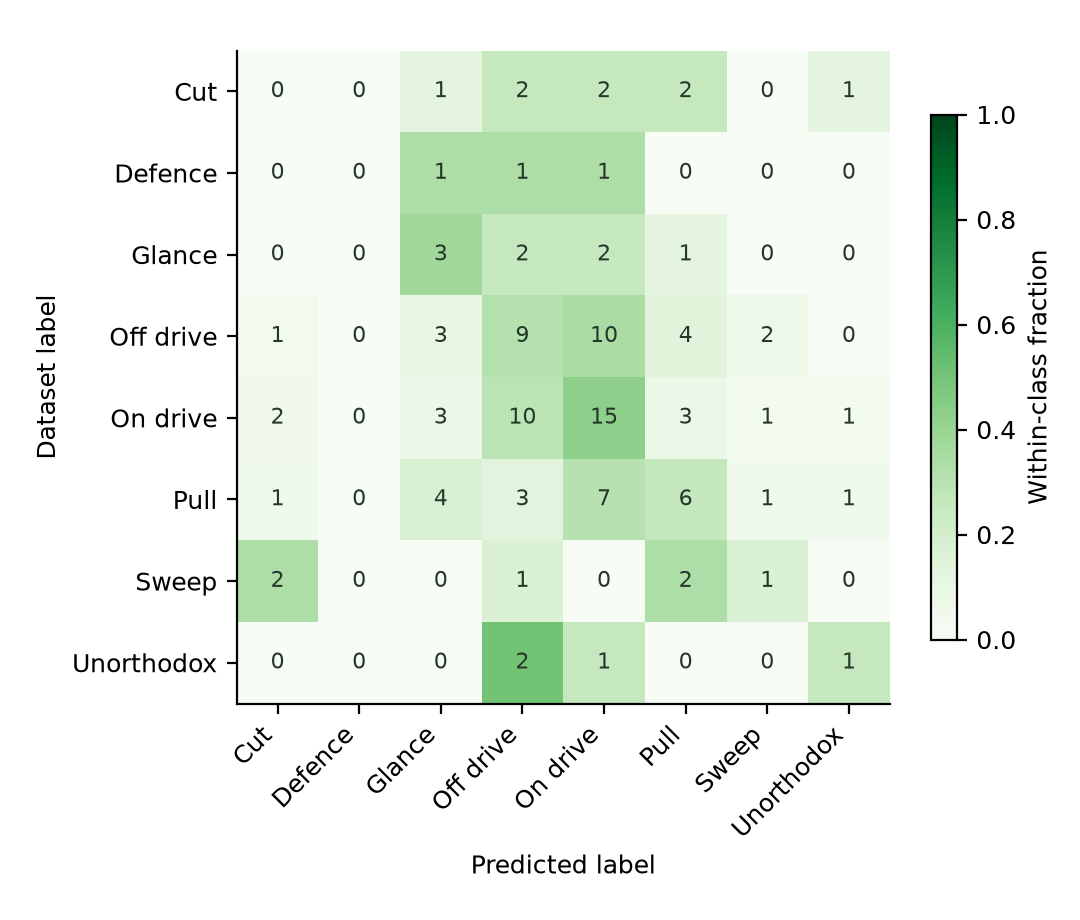
\includegraphics[width=\linewidth]{confusion_matrix.png}
\caption{Proposed model on the complete test split. Numbers are clip counts. Color shows row-normalized fractions.}
\label{fig:confusion}
\end{figure}

Figure~\ref{fig:confusion} shows uneven class behavior. On drive recall is 42.9\% on 35 clips, while cut recall is 0.0\% on 8. Defence has only three test clips, so one changed prediction moves its recall by 33.3 points. The single unorthodox validation clip also makes class-specific tuning unreliable. The apparent difference between models should not be treated as a statistically established improvement. A 2,000-draw source-group bootstrap gives an accuracy interval of 25.0--35.2\% and macro F1 interval of 16.6--31.0\% for the proposed model. Only 5 independent test groups contribute to this resampling. The intervals condition on this trained model and omit training and split variability.

\subsection{Calibration and selective prediction}
\begin{table}[t]
\centering\small
\begin{tabular}{lrrr}
\toprule
Probabilities & NLL & ECE & Brier \\
\midrule
Before calibration & 2.054 & 0.204 & 0.914 \\
After calibration & 1.885 & 0.105 & 0.843 \\
\bottomrule
\end{tabular}
\caption{Proposed model on test clips. ECE uses ten equal-width confidence bins. Brier is the unscaled mean sum of squared errors over eight classes. Lower is better.}
\label{tab:cal}
\end{table}

The fitted temperature is 1.760 and the review threshold is 0.80. No candidate met the stated validation target, so the 0.80 fallback was used. On test clips, the rule accepts 0 of 116 (0.0\% coverage), with accepted accuracy undefined because no clip is accepted. This operating result is an observation, not a promised 90\% accuracy. Temperature scaling leaves the confusion matrix unchanged. A calibrated score is still not evidence that an unknown upload belongs to one of the eight classes.

\begin{figure}[t]
\centering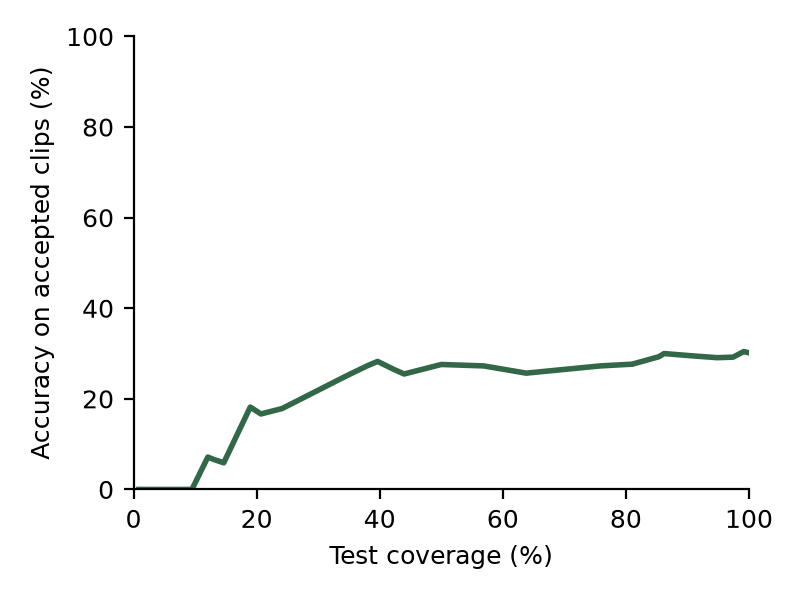
\includegraphics[width=\linewidth]{selective_curve.png}
\caption{Coverage versus accuracy on the test split. The operating threshold was chosen on validation data. Other points are descriptive test diagnostics and are not threshold tuning.}
\end{figure}

\subsection{Temporal reversal and corruption}
\begin{table}[t]
\centering\small
\begin{tabular}{lrrrr}
\toprule
Representation & Clean & Dark & Blur & Reverse \\
\midrule
Middle frame & 19.8 & 20.7 & 19.0 & 19.8 \\
Temporal mean & 18.1 & 21.6 & 7.8 & 18.1 \\
Phase + diff./std. & 30.2 & 25.0 & 23.3 & 12.9 \\
\bottomrule
\end{tabular}
\caption{Test accuracy in percent. Every corruption uses the complete unchanged test set. Reverse changes temporal order only.}
\label{tab:robust}
\end{table}

We reverse the order of cached test embeddings without retraining to probe dependence on chronology. Mean pooling is invariant by construction. The proposed model changes from 30.2\% to 12.9\% accuracy. The drop is consistent with some use of temporal order, but it does not identify which movements the model recognizes. Reversal is a mechanism diagnostic, not a realistic deployment distribution.

For two visual stress tests, we multiply frame brightness by 0.6 and apply Gaussian blur of radius two at preview resolution. We recompute embeddings for every test clip and keep the classifier fixed. The proposed model scores 25.0\% in the darkened condition and 23.3\% under blur. Neither corruption result is used to retrain or select the model. These transformations are narrow stress tests. They do not establish robustness to a new camera, background, tournament or unseen shot category.

\subsection{Failure analysis and runtime}
\begin{figure}[t]
\centering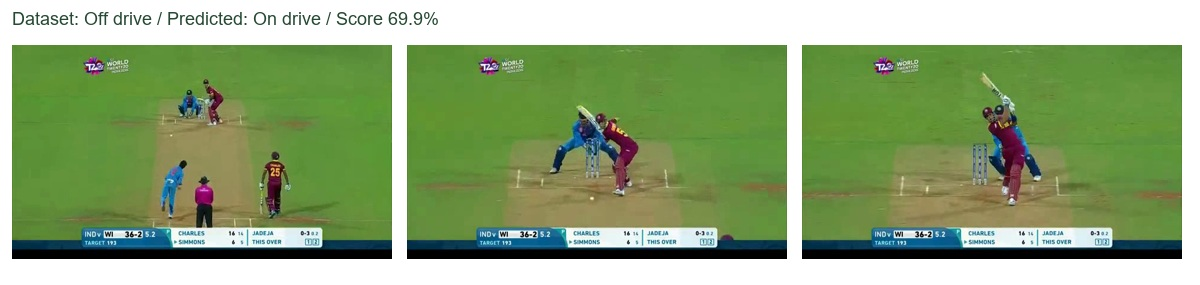
\includegraphics[width=\linewidth]{failure_example.jpg}
\caption{A selected confident error, shown after evaluation. The title identifies the dataset label, prediction and score. Selected examples are not a representative estimate of performance.}
\label{fig:failure}
\end{figure}
Figure~\ref{fig:failure} is clip \texttt{clip\_0239}, whose upstream label is off drive. The model predicts on drive with score 69.9\%. We deliberately include this confident error in the demo rather than showing only successful clips. We cannot infer the exact cause of this mistake from a frame strip. Background correlations, weak motion evidence and label ambiguity are plausible explanations that would require further annotation to distinguish.

End-to-end inference on 25 deterministic test clips takes 88 ms at the median and 91 ms at the 95th percentile on the recorded host. Timing includes decoding, sampling, nine encoder passes and the classifier, with one warm-up and model construction excluded. It describes this machine and these short clips, not a real-time guarantee.

\section{Demo and practical limitations}
The local Flask interface accepts a trimmed video up to 30 seconds and 40 MB. It displays the top candidate, all eight calibrated scores, three groups of sample frames and a review decision. Uploaded files use temporary storage and do not leave the computer. Downloadable JSON records the result. Bundled test examples include successful predictions, a confident error and a low-confidence clip, all marked as selected after evaluation.

The system requires a pre-trimmed single shot. It does not localize a batter or contact frame. The archive is small, imbalanced and limited to its own broadcast sources. We have not independently audited every label, measured player-level generalization or evaluated non-cricket rejection. Low confidence can help request review, but high confidence can still accompany a wrong or out-of-scope input. The current validation set is also too small to support a promised error rate.

Useful next experiments would annotate player and camera identities, separate calibration data from model-selection data, obtain more defence and unorthodox examples, and compare a trainable temporal head under the same source split. A detector-based batter crop could reduce background cues, but this implementation does not include one.

\section{Conclusion}
The proposed representation exceeds the middle-frame macro F1 by 2.7 percentage points. The ablations show how much of the result survives changes in temporal representation and input quality. Because the ROI revision followed pilot test feedback, the results should guide a larger independent evaluation rather than serve as a final generalization claim. The main deliverable is a working and inspectable video-recognition pipeline with a traceable evaluation. Its results support a limited claim about eight labels in a held-out portion of this archive. They do not establish general cricket understanding or coaching reliability.

\section*{Submission information}
The group will choose and publish its GitHub repository after reviewing the project. The required repository URL is not yet available and must be inserted before submission.
The complete source listing follows the references in the full report. Data, pretrained weights, library repositories and the template source are linked in Appendix A and in the accompanying source register. Individual names and specific contributions remain for the five group members to supply; no contribution claims have been fabricated.
